\documentclass{beamer}
\usepackage{HECbeamer}
% \usepackage{pgfpages}
% \pgfpagesuselayout{4 on 1}[letterpaper, landscape, border shrink=5mm]
\title[\color{white}{MATH 60604 \S~7c - Estimateur de Kaplan--Meier}]{\texorpdfstring{MATH 60604 \\Modélisation statistique \\ \S~7c - Estimateur de Kaplan$-$Meier}{MATH 60604 \\ Modélisation statistique \\ \S~7c - Estimateur de Kaplan-Meier}}
\author{Léo Belzile}
\institute{HEC Montréal\\
Département de sciences de la décision}
\date{} 

\begin{document}
\frame{\titlepage}
% \begin{frame}
% \frametitle{Estimateur Kaplan--Meier}
% \begin{itemize}
% % \item Les méthodes d'analyse de survie sont spécifiquement conçues pour être en mesure de bien prendre en compte de la censure.
% \item L'un des estimateurs les plus couramment utilisés pour estimer la fonction de survie en présence de censure à droite non-informative est l'estimateur de \alert{Kaplan--Meier}.
% \item L'estimateur de Kaplan--Meier  est \alert{non-paramétrique}, c'est-à-dire, on ne fait pas d'hypothèse sur la loi de probabilité sous-jacente de la variable réponse $T_i$.
% \end{itemize}
% %    
% % \item \footnotesize{Notez qu'il existe de nombreuses méthodes pour estimer les courbes de survie. Par exemple, certains modèles paramétriques comprennent le modèle de Weibull, le modèle log-normal, etc. Nous ne verrons pas ces modèles.}
% 
% \end{frame}

\begin{frame}
\frametitle{Notation}
On considère $T$ une variable aléatoire continue et un échantillon de taille $n$.
\begin{itemize}
%\item Suppose we have $n$ subjects, for which we either observe the time until the event, or a (right) censored time.
\item Supposons qu'il y a $D$ temps distincts de défaillance. 
\item Soit $0 \leq t_1 < t_2 < \cdots < t_D$ ces $D$ temps en ordre croissant. 
\item Soit $r_j$ le nombre d'individus \emph{à risque} d'expérimenter l'événement au temps $t_j$ . 
\bi
\item C'est-à-dire, ces individus n'ont toujours pas expérimenté l'événement (et n'ont pas été censuré) avant le temps $t_j$. 
\item Donc, $r_j$ est le nombre de survivants juste avant le temps $t_j$ qui sont à risques d'expérimenter l'événement au temps $t_j$.
\ei
\item Soit $d_j \in \{0, \ldots, r_j\}$ le nombre d'individus qui expérimentent l'événement au temps $t_j$ (par exemple, il y a $d_j$ décès au temps $t_j$). 
\end{itemize}
\end{frame}
\begin{frame}
\frametitle{Dérivation de l'estimateur de Kaplan--Meier}
 La probabilité de mourir dans l'intervalle $(t_j, t_{j+1}]$ étant donné que l'individu a survécu jusqu'à $t_j$ est 
 \begin{align*}
  h_j = \P{t_j < T \leq t_{j+1} \mid T > t_j} 
%   \\& = \frac{\P{t_j < T \leq t_{j+1}}}{\P{T > t_j} }
%   \\& 
  = \frac{S(t_j) - S(t_{j+1})}{S(t_j)}.
 \end{align*}
d'où une récursion qui donne \begin{align*}
S(t) = \prod_{j: t_j < t} (1-h_j).
\end{align*}
L'estimateur de Kaplan--Meier  est \alert{non-paramétrique}, 
\bi \item on ne fait pas d'hypothèse sur la loi de probabilité sous-jacente de  $T_i$.
\item on considère plutôt les $\{h_j\}_{j=1}^D$ comme des paramètres du modèle.
\ei
\end{frame}

\begin{frame}
\frametitle{Vraisemblance pour données discrètes}
\bi \item Chacun des décès au temps $t_j$ contribue $h_j$ à la vraisemblance 
\bi \item la probabilité de défaillance à $t_j$ sachant qu'un individu a survécu jusque là. \ei 
\item 
Les survivants au temps $t_j$ contributent $1-h_j$.
\item 
On peut donc écrire la vraisemblance comme
\begin{align*}
 \ell(\bs{h}) = \sum_{j=1}^D \{ d_j \ln(h_j) + (r_j-d_j)\ln(1-h_j)\},
\end{align*}
soit la somme des contributions de variables binomiales du risque au temps $t_j$.
\ei
\end{frame}
\begin{frame}
\frametitle{Optimisation des différents probabilité de survie}
\begin{itemize}
\item Si on différencie $\ell(\bs{h})$ par rapport à $h_j$, on trouve $\widehat{h}_j = d_j/r_j$.
\item L'estimateur de Kaplan--Meier pour la fonction de survie est
\begin{align*}
\widehat{S}(t) = \prod_{t_j < t} \left( 1 - \frac{d_j}{r_j} \right)                                                                      \end{align*}
\item 
Intuition: $d_j/r_j$ représente la probabilité conditionnelle de survivre jusqu'avant le temps $t_j$ et d'expérimenter l'événement au temps $t_j$. 
\end{itemize}
\end{frame}

\begin{frame}
\frametitle{Exemple}
 Les données \code{cancersein} tirées de Sedmak \textsl{et al.} (1989) traitent de survie de patients atteints du cancer du sein et contiennent les variables suivantes:
\begin{itemize}
 
\item \code{temps}: temps de survie ou temps écoulé à la fin de l'étude (en mois)
\item \code{mort}: variable indicatrice pour la mort, \code{0} pour censure, \code{1} pour décès
\item \code{repimmuno}: réaction à un examen immunohistochimique, soit négative (\code{0}) ou positive (\code{1})
\end{itemize}
%    
% 
% \item[] \tiny{
% Ces données proviennent de (), comme l'illustre le livre \emph{Survival Analysis: Techniques for Censored and Truncated Data} par John P. Klein \& Melvin L. Moeschberger}
% \end{itemize}
\end{frame}


\begin{frame}
\frametitle{Statistiques descriptives pour \code{cancersein}}
\begin{center}
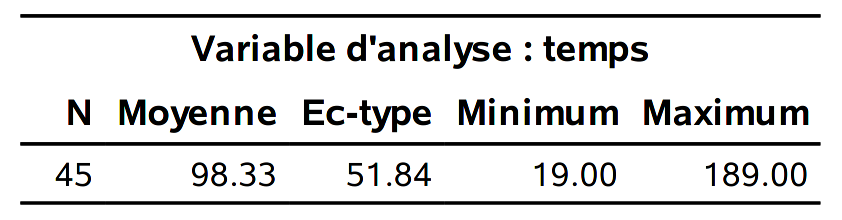
\includegraphics[width = 0.5\textwidth]{img/c7/diapos7e01}
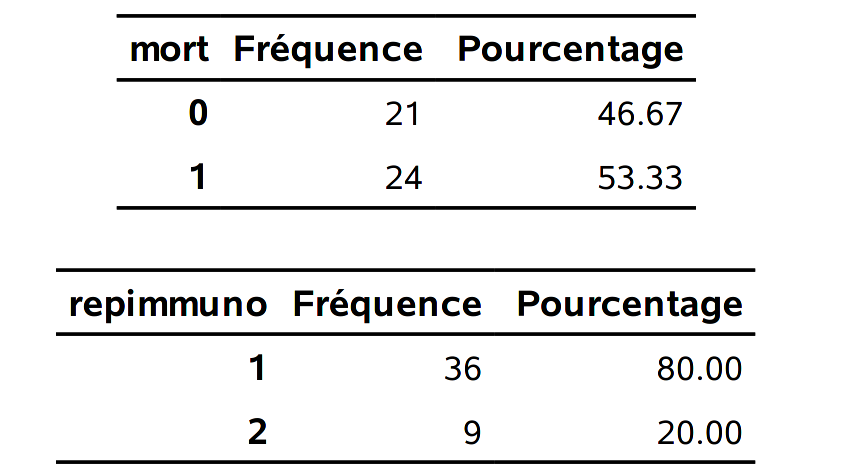
\includegraphics[width = 0.5\textwidth]{img/c7/diapos7e02}
\end{center}
{
\footnotesize En pratique, l'utilisation de l'estimateur de Kaplan--Meier avec si peu de données est déconseillée. La qualité de l'approximation dépend fortement du nombre d'observations (correct si $n \gg 1000$).

Les observations censurées fournissent beaucoup moins d'observations que les temps de défaillance observés.

}
\end{frame}


\begin{frame}[fragile]
\frametitle{Estimation de la fonction de survie }

\begin{tcolorbox}[colback=white,colframe=hecblue,title=Code \SASlang{} pour ajuster l'estimateur de Kaplan--Meier]
{\footnotesize 
\begin{verbatim}
proc lifetest data=modstat.cancersein method=km plots=(s(cl));
time temps*mort(0);
run;
\end{verbatim}
}
\end{tcolorbox}
{ \footnotesize 
L'argument \code{time} indique la variable de temps $T$ (\code{temps}) et l'indicateur de censure,  incluant la valeur de référence pour les observations censurées à droite (\code{mort=0})

}
\end{frame}

\begin{frame}
\frametitle{Estimé de la fonction de survie}
\begin{center}
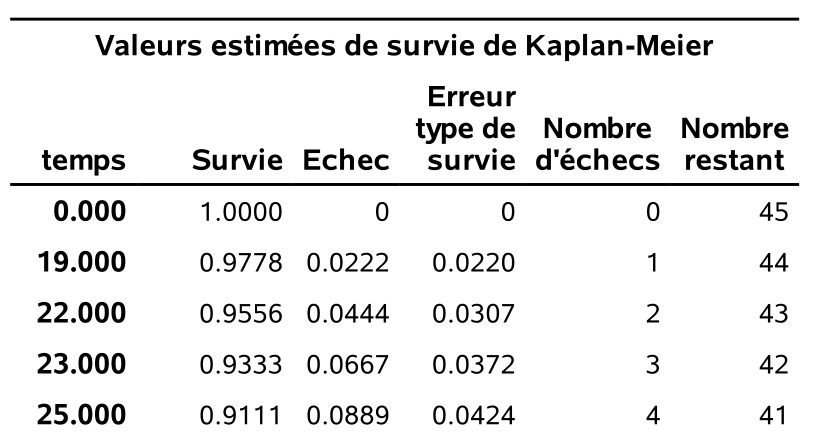
\includegraphics[width = 0.6\textwidth]{img/c7/diapos7e03}
\begin{align*}
 \vdots
\end{align*}
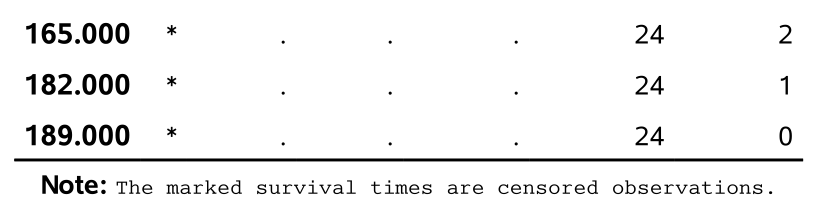
\includegraphics[width = 0.6\textwidth]{img/c7/diapos7e04}
\end{center}
\end{frame}

\begin{frame}
\frametitle{Graphique de la fonction de survie}
\begin{center}
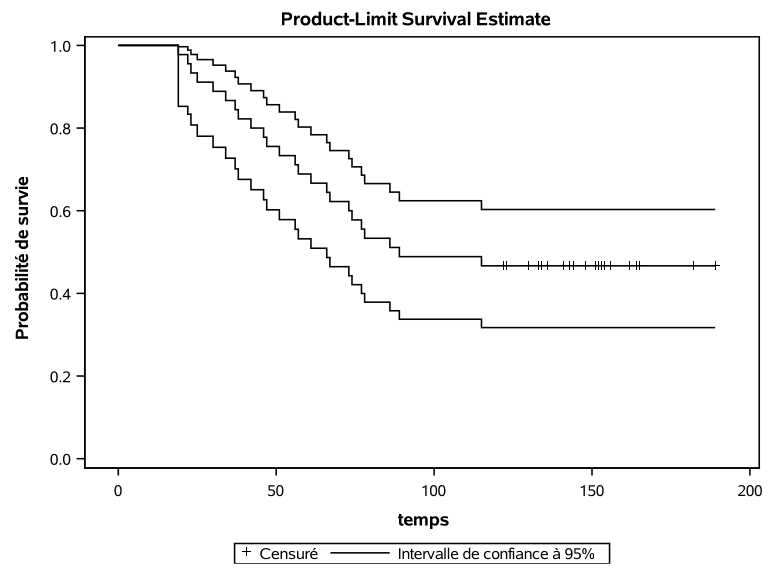
\includegraphics[width = 0.8\textwidth]{img/c7/diapos7e05}
\end{center}
{ \footnotesize 

La courbe de survie estimée est déficiente: $\widehat{S}(t)$ ne descend jamais à $0$ parce que le temps de survie le plus long dans les données est censuré à droite.


}
\end{frame}
% \begin{frame}
% \bi \bi
% \item On voit que la dernière observation de temps à $t=189$ est représenté par une coche dans le graphique car l'observation est censurée. 
% \item La dernière baisse de $\widehat{S}(t)$ sera à $t_D$: le plus grand temps de décès observé.  
% 
% \begin{center}
% \includegraphics[scale=0.6]{img/c7/btrial_plateau.png}
% \end{center}
% 
% \end{itemize}
% \end{itemize}
% \end{frame}

\begin{frame}
\frametitle{Durée de l'allaitement}
La base de données \code{allaitement} contient des données provenant de l'Enquête longitudinale nationale sur les jeunes sur la durée de la période d'allaitement de mères depuis la naissance de leur bébé. On se concentre sur les variables suivantes:
\begin{itemize}
\item \code{duration}: durée de l'allaitement (en semaines)
\item \code{delta}: variable indicatrice de la fin de l'allaitement, 
\bi \item soit observée (\code{1}) 
\item soit censurée (\code{0})
\ei
%\item \code{race}: race of mother (1=white, 2=black, 3=other)
%\item \code{poverty}: poverty status of mother (1=yes, 0=no)
%\item \code{smoke}: smoking status of mother at birth of child (1=yes, 0=no)
%\item \code{alcohol}: alcohol-drinking status of mother at birth of child (1=yes, 0=no)
%\item \code{agemth} age of mother at birth of child
%\item \code{ybirth} year of child's birth
%\item \code{yschool}: education level of mother (years of school)
%\item \code{pc3mth}: lack of prenatal care status (1= mother did not seek within first 3 months, 0=mother sought prenatal care in first three months of pregnancy)

\end{itemize}
\begin{center}
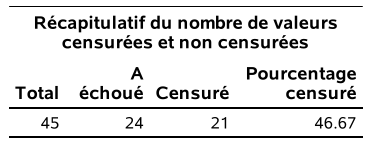
\includegraphics[width = 0.5\textwidth]{img/c7/diapos7e06}
\end{center}
% 
% \item[] \tiny{Ces données proviennent de l'Enquête longitudinale nationale sur les jeunes, tels qu'illustrés dans le livre \emph{Survival Analysis: Techniques for Censored and Truncated Data} par John P. Klein \& Melvin L. Moeschberger}
% \end{itemize}
\end{frame}

\begin{frame}
\frametitle{Courbe de survie pour les données \code{allaitement}}

\begin{center}
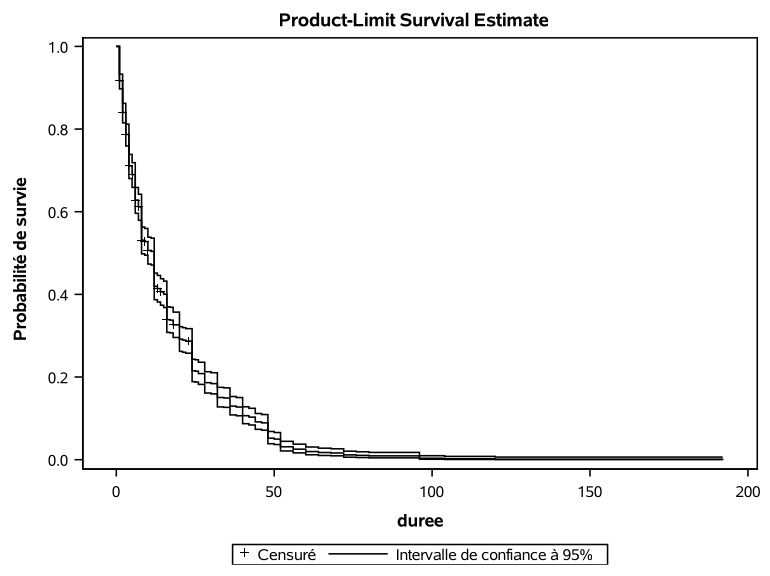
\includegraphics[width = 0.8\textwidth]{img/c7/diapos7e08}
\end{center}
{\footnotesize $\widehat{S}(t)$ atteindra zéro puisque le plus grand temps de survie est observé.

}
\end{frame}
% 
% \begin{frame}
% \frametitle{Exemple}
% \begin{itemize}
% \item Dans cet exemple, la courbe de survie estimée atteint $0$. 
% \item C'est parce que le temps de survie le plus grand dans les données n'est pas censuré:
% 
%     
% 
% %\begin{center}
% \begin{tabular}{c c}
% %\begin{footnotesize}
% \code{duration} & \code{delta} \\
% 192 &  1
% %\end{footnotesize}
% \end{tabular}
% %\end{center}
% 
% \item La dernière baisse dans $\widehat{S}(t)$ atteindra zéro puisque le plus grand temps de survie observé dans les données est en fait le dernier temps d'événement $t_D$.  
% 
% \begin{center}
% \includegraphics[scale=0.6]{img/c7/bfeed_plateau.png}
% \end{center}
% 
% \end{itemize}
% \end{frame}

\begin{frame}[fragile]
\frametitle{La médiane de survie}
 La médiane du temps de survie est le temps $t_M$ auquel $S(t_M)=0.5$. 
\begin{itemize}
 \item C'est-à-dire, le temps médian $t_M$ est tel que $50\%$ des individus survivent jusqu'au temps $t_M$. 
\end{itemize}
 On peut facilement trouver la médiane du temps de survie en cherchant le temps $t$ o\`u la ligne horizontale $S(t) = 0.5$ croise la courbe de survie. 
\begin{center}
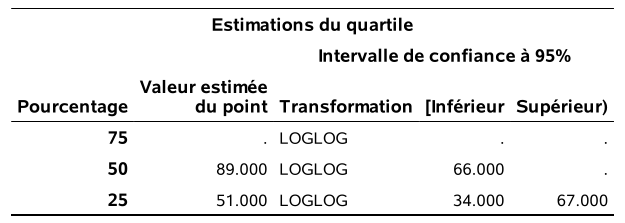
\includegraphics[width = 0.7\textwidth]{img/c7/diapos7e07}
\end{center}

\end{frame}

% \begin{frame}[fragile]
% \frametitle{La médiane de survie}
% \begin{itemize}
% \item SAS va automatiquement calculer la médiane du temps de survie. 
% \item Dans les données sur les patients avec le cancer du sein, on obtient un temps de survie médian de $89$
%   
% \begin{center}
% \includegraphics[scale=0.4]{img/c7/btrial_km_median.png}
% \end{center}
% \item Notez que si le temps observé le plus long est \alert{censuré} et que la courbe de survie estimée atteint un plateau qui est plus \alert{élevé} que la ligne horizontale de $0.5$, alors nous ne pourrons pas estimer la médiane du temps de survie. 
% \begin{center}
% \includegraphics[scale=0.35]{img/c7/km_ex_no_med.png}
% \end{center}
% \end{itemize}
% \end{frame}


\begin{frame}
\frametitle{Moyenne de la survie}
Pour une variable aléatoire positive, $T>0$, on peut démontrer que 
\begin{align*}
\E{T} = \int_0^{\infty} S(t) \d t
\end{align*}
On peut estimer l'espérance du temps de survie $\E{T}$ en calculant l'aire sous la courbe de survie estimée $\widehat{S}(t)$. 
\begin{itemize}
\item Par exemple, le temps de survie moyen pour les données d'allaitement est $16.89$ semaines avec erreur-type $0.614$ semaines.
\item Si le temps observé le plus long est \alert{censuré}, la courbe de survie estimée $\widehat{S}(t)$ va atteindre un plateau et ne descendra jamais à $0$.
\item Dans ce cas, on peut plutôt estimer le temps de survie moyen limité: $\E{\min\{T,\tau\}}$ pour une valeur choisie $\tau$. C'est-à-dire, nous calculerons le temps de survie moyen comme si la courbe descendait à $0$ au temps $\tau$ (option \code{rmst} dans \SASlang{}).
\end{itemize} 
\end{frame}
% 
% \begin{frame}
% \frametitle{Exemple}
% %\textbf{SAS output}
% \begin{itemize}
% \item Par défaut, \SASlang{} va estimer la moyenne du temps de survie o\`u l'estimation est limitée au plus grand temps d'événement observé $t_D$.
% \item Ex: pour les données sur les patients avec le cancer du sein, on obtient
%   
% \begin{center}
% \includegraphics[scale=0.5]{img/c7/btrial_km_mean.png}
% \end{center}
% \item Remarquez que SAS indique que la moyenne du temps de survie est \alert{sous-estimée} puisque l'estimation est limitée au plus grand temps d'événement, mais dans les données la plus grande observation est censurée\ldots
% \end{itemize}
% \end{frame}
% % 
% \begin{frame}[fragile]
% \frametitle{Exemple}
% \begin{itemize}
% \item Si on inclut l'option \code{rmst} en SAS, la moyenne limitée sera calculée, et l'estimation sera limitée à la plus grande valeur observée $t_{max}$, ou à un $\tau$ spécifié. 
% \end{itemize}
% \begin{tcolorbox}[colback=white,colframe=blue!75!black,title=Code SAS ]
% \begin{verbatim}
% proc lifetest data=modstat.btrial method=km
% plots=(s(cl)) rmst;
% time time*death(0);
% run;
% \end{verbatim}
% \end{tcolorbox}
% \begin{center}
% \includegraphics[scale=0.5]{img/c7/btrial_rmst.png}
% \end{center}
% \begin{itemize} 
% \item On voit que SAS sélectionne $\tau=189$, qui est le plus grand temps dans l'ensemble de données (observation censurée).
% \end{itemize}
% \end{frame}

\end{document}
